\chapter{Theory}

\section{MOT Physics}

brief overview of zeeman slower, mot

\section{Electron Generation in the Cold-Atom Electron Source}
The \gls{caes} uses two stage photoionisation as its primary method of electron production. This method provides strong control over the excess energy of the ionised electrons which is essential to the production of cold electrons. Control of the initial electron bunch shape is also possible as described by McCulluch et. al. \cite{mcculloch_arbitrarily_2011}.

Two lasers with different wavelengths can be used for efficient ionisation of atoms while producing cold electrons. An excitation laser takes the atoms from the ground state to an intermediary excited state and an ionisation laser takes the excited atoms from the intermediary state to the ionisation continium. The excess energy of the ionised electrons can be controlled by varying the wavelength of the ionisation laser.

\begin{figure}
\centering
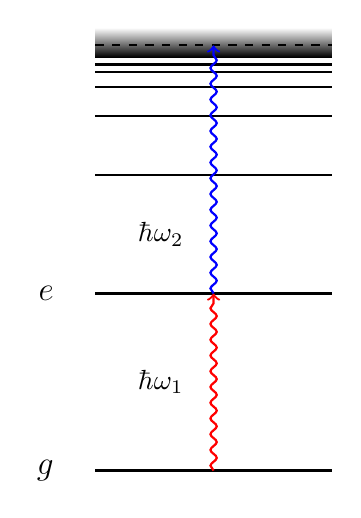
\begin{tikzpicture}[scale=1.5]
    \begin{scope}[thick, decoration={snake,amplitude=.4mm,
        segment length=2mm,post length=1mm}]
      \draw (0, 0) node[left=0.4cm] {\large $\ket{g}$}
        -- (2, 0);
      \draw (0, 1.5)  node[left=0.4cm] {\large $\ket{e}$}
        -- (2, 1.5);

      \draw (0, 2.5) -- (2, 2.5);
      \draw (0, 3) -- (2, 3);
      \draw (0, 3.25) -- (2, 3.25);
      \draw (0, 3.375) -- (2, 3.375);
      \draw (0, 3.4375) -- (2, 3.4375);
      \draw (0, 3.5) -- (2, 3.5);
      \shade[top color=white,bottom color=black] (0, 3.5) rectangle (2, 3.75);

      \draw[style=dashed] (0, 3.6) -- (2, 3.6);

      \draw[decorate,red,->] (1,0) -- ++(90:1.5);% excitation
      \draw[decorate,blue,->] (1,1.5) -- ++(90:2.1);% ionisation

      \draw (1, 0.75) node[left=0.25cm] {$\hbar\omega_1$};
      \draw (1, 2) node[left=0.25cm] {$\hbar\omega_2$};
    \end{scope}
\end{tikzpicture}
\caption[Title]{Energy level diagram for atom undergoing two-stage ionisation. Resonant excitation from the ground state, $\ket{g}$ to the excited state $\ket{e}$ is achieved with a coupling laser of frequency $\omega_1$. A second laser of frequency $\omega_2$is used to couple $\ket{e}$ to the ionisation continuum. Changing $\omega_2$ allows the excess energy of the ionisation process to be adjusted.}
\label{fig:energy_level}
\end{figure}

In the \gls{caes} the excitation laser is resonant to the D2 transition of the trapped $^{85}$Rb atoms (780.24nm). This resonance results in efficient population transfer to the excited state. The ionisation laser can be set to couple the first excited state to a Rydberg state rather than to the ionisation continuum directly which results in resonant transitions. The resonant transition to a Rydberg state followed by field ionisation induced by the accelerating electric field (see figure \ref{fig:field_ionisation}) is more efficient than other ionisation pathways which rely on non-resonant behaviour. Field ionisation results in free electrons with very little energy ($T\approx10K$\cite{mcculloch_arbitrarily_2011}) and are thus called `cold'.

\begin{figure}
\centering
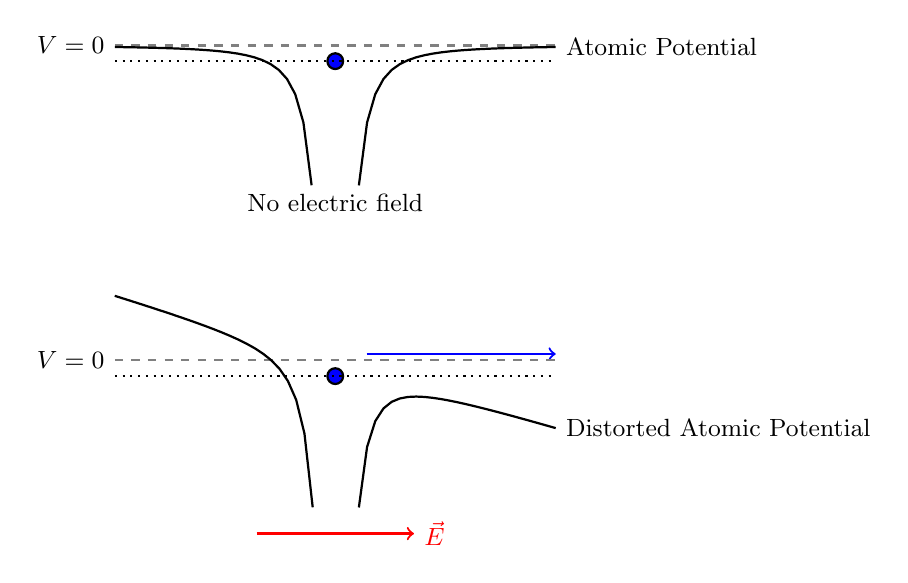
\begin{tikzpicture}[scale=2]
    \begin{scope}[thick, decoration={snake,amplitude=.4mm,
        segment length=2mm,post length=1mm}]

    \filldraw[fill=blue] (0, 1.9) circle (0.05);
    \draw [color=black, dotted] (-1.4, 1.9) -- (1.4, 1.9);
    \draw (0, 1) node {\small No electric field};
    \draw [dashed, color=gray] (-1.4, 2) node[color=black, left] {\small $V=0$} -- (1.4, 2);

    \draw[domain=-1.4:-0.15, color=black] plot (\x, {-1/(50*\x*\x)+2});
    \draw[domain=0.15:1.4, color=black] plot (\x, {-1/(50*\x*\x)+2}) node[right] {\small Atomic Potential};

    \filldraw[fill=blue] (0, -0.1) circle (0.05);
    \draw [color=black, dotted] (-1.4, -0.1) -- (1.4, -0.1);
    \draw [color=blue, above=4, ->] (0.2, -0.1) -- (1.4, -0.1);
    \draw [color=red, ->] (-0.5, -1.1) -- (0.5, -1.1) node [right] {\small $\vec{E}$};
    \draw [dashed, color=gray] (-1.4, 0) node[color=black, left] {\small $V=0$} -- (1.4, 0);

    \draw[domain=-1.4:-0.143, color=black] plot (\x, {-1/(50*\x*\x)-0.3*\x});
    \draw[domain=0.15:1.4, color=black] plot (\x, {-1/(50*\x*\x)-0.3*\x}) node[right] {\small Distorted Atomic Potential};

    \end{scope}
\end{tikzpicture}
\caption[Title]{The top diagram dipicts an atom excited to a Rydberg state without the presence of an electric field. The lower diagram show the same atom in the presence of an electric field. The electric field distorts the atomic potential in such a way as to allow the atom to become ionised. The solid black lines represent the atomic potential, the dashed lines the zero field ionisation threshhold, the dotted lines the energy of the valence electrons, the blue circles show the elctrons and the red arrow the direction of the electric field.}
\label{fig:field_ionisation}
\end{figure}

The cold electrons are then accelerated with an electric field and steered with a number of magnetic devices through the sample and onto the detector.

\section{Optical Dipole Traps}

The following derivation of the dipole potential and scattering rate for \gls{odt} follows the one presented in Grimm and Weidem\"uller\cite{grimm_optical_2000}.

An electric field, $\emph{E}$, from laser light of frequency $\omega$ will induce an atomic dipole moment $\boldsymbol{p}$ in an atom placed within the light field. Using standard complex notation we can write,

\begin{equation}\label{eq:efield}
\boldsymbol E (\boldsymbol r ,t)=\hat{\boldsymbol e} \tilde E (\boldsymbol r) \exp{-i\omega t + c.c.}
\end{equation}
where $\hat{\boldsymbol{e}}$ is the polarisation unit vector. The amplitude of the dipole moment, $\tilde p$, is related to the electric field amplitude, $\tilde E$, by
\begin{equation}\label{eq:polarisability}
\tilde p = \alpha \tilde E.
\end{equation}
$\alpha$ depends on the driving frequency, $\omega$ and is called the complex polarisability.

The induced dipole moment, $\boldsymbol p$ has an interaction potential with the electric field, $\boldsymbol E$ given by
\begin{equation}\label{eq:interaction_pot}
U_{dip} = - \frac{1}{2} \langle \boldsymbol{pE} \rangle = - \frac{1}{2 \epsilon_0 c} Re(\alpha)I,
\end{equation}
where the time average over the rapidly oscillating terms is indicated by the angle brackers, the field intensity is $I=2\epsilon_0 c |\tilde E|^2$ and the $\frac{1}{2}$ takes the the induced nature of the dipole moment in account. The dipole force results from the gradient of the interaction potential
\begin{equation}\label{eq:dipole_force}
\boldsymbol F_{dip}(\boldsymbol r ) = - \nabla U_{dip}(\boldsymbol r) = \frac{1}{2 \epsilon_0 c} Re(\alpha) \nabla I(\boldsymbol r).
\end{equation}
The dipole force is a conservative force and is proportional to gradient of the intensity of the light field.

The oscillator absorbs power from the light field which is re-emitted as dipole radiation. This is given by,

\begin{equation}\label{eq:power_absorbed}
P_{abs} = \langle \boldsymbol{\dot p E} \rangle = 2 \omega Im(\tilde p \tilde E^*) = \frac{\omega}{\epsilon_0 c} Im (\alpha) I
\end{equation}

The complex part of the polarisability gives the out of phase component of the dipole oscillation which results in absorption. Absorption can be interpreted in terms of photon scattering in cycles of absorption and emission of photons of energy $\hbar \omega$. This corresponds to a scattering rate of
\begin{equation}\label{eq:scattering_rate}
\Gamma(\boldsymbol r) = \frac{P_{abs}}{\hbar \omega} = \frac{1}{\hbar \epsilon_0 c} Im(\alpha) I(\boldsymbol r).
\end{equation}

\subsection{Atomic Polarisability}

The atomic polarisability, $\alpha$ can be calculated by using Lorentz's model for a classical oscillator {\color{red} citation please}. In this picture an electron with mass $m_e$ and charge $e$ is considered to be bounds to the core elastically with an oscillation frequency $\omega_0$ which corresponds to the optical transition frequency.

The polarisability can be calculated if the equation of motion, $\ddot{x} + \gamma \dot{x} + \omega_0^2 x = -eE(t)/m_e$, is integrated for the driven oscillation of the electron to give
\begin{equation} \label{eq:polarisability}
\alpha = \frac{e^2}{m_e} \frac{1}{\omega_0^2-\omega^2-i\omega\Gamma_\omega}
\end{equation}
where the damping rate due to radiative energy loss is
\begin{equation}\label{eq:damping_rate}
\Gamma_\omega=\frac{e^2\omega^2}{6\pi\epsilon_0m_ec^3}.
\end{equation}
By substituting $e^2/m_e=6\pi\epsilon_0 c^3\Gamma_\omega / \omega^2$ and the on-resonance damping rate $\Gamma \equiv \Gamma_{\omega_0} = (\omega_0/\omega)^2\Gamma_\omega$ we get
\begin{equation}\label{eq:final_polarisability}
\alpha = 6\pi \epsilon_0 c^3 \frac{\Gamma/\omega_0^2}{\omega_0^2 - \omega^2 - i(\omega^3/\omega_0^2)\Gamma}
\end{equation}

While this is classically derived is serves as a good approximation for far-detuned dipole traps due to the relatively low scattering rates and hence low saturation\cite{grimm_optical_2000}.

\subsection{Optical Dipole Force and Scattering Rate}

Using equation \ref{eq:final_polarisability} in \ref{eq:interaction_pot} and \ref{eq:scattering_rate} in the case of large detuning and negligible saturation we can derive

\begin{equation}\label{eq:potential}
U_{dip}(\boldsymbol r) = -\frac{3\pi c^2}{2\omega_0^3}\left(\frac{\Gamma}{\omega_0-\omega} + \frac{\Gamma}{\omega_0+\omega}\right) I(\boldsymbol r),
\end{equation}
and
\begin{equation}\label{eq:scattering}
\Gamma_{sc} = \frac{3\pi c^2}{2\hbar\omega_0^3} \left(\frac{\omega}{\omega_0}\right)^3 \left(\frac{\Gamma}{\omega_0 - \omega} + \frac{\Gamma}{\omega_0+\omega}\right)^2 I(\boldsymbol r).
\end{equation}

Most experiments are performed with $\omega$ relatively close to the resonance, $\omega_0$. In this case the detuning $\Delta\equiv \omega - \omega_0 \ll \omega_0$. Here we can make the rotating wave approximation and set $\omega/\omega_0\approx 1$. The equations above simplify to

\begin{equation}\label{eq:simple_potential}
U_{dip}(\boldsymbol{r}) = \frac{3\pi c^2}{2 \omega_0^3} \frac{\Gamma}{\Delta} I(\boldsymbol{r}),
\end{equation}
and
\begin{equation}\label{eq:simple_scattering}
\Gamma_{sc} (\boldsymbol r ) = \frac{3\pi c^2}{2\hbar\omega_0^3} \left( \frac{\Gamma}{\Delta} \right)^2 I(\boldsymbol r ).
\end{equation}

These equations provide the basis for understanding the operation of dipole traps. The sign of the detuning is clearly important. For below resonance or `red' detuning ($\Delta < 0$) the dipole potential is negative and atoms are drawn into the high intensity portions of the light field. Above resonance or `blue' detuning ($\Delta > 0$) results in repulsion from the high intensity regions of the light and a positive potential.

The potential scales with $I/\Delta$ and the scattering scales with $I/\Delta^2$ which means that for a certain potential depth high intensity and detuning will result in the least scattering.

{\color{red} Still need to talk about how these equations make a trap as well as some theoretical numbers}

\subsection{lifetime}

{\color{red} hmmm what to do here....}

\subsection{Configuration}

remember to mention polarisation stuff for the crossed beam trap

\section{Imaging}

In order to determine the spatial state of the atoms at a given time techniques for imaging are required. Numerous techniques for imaging have been developed the simplest of which are fluorescence and absorption imaging.

\subsection{Fluorescence Imaging}

Near resonant light passing through atom clouds (such as the optical mollasses lasers in a \gls{mot} or a specific probe beam) will be absorbed and re-emitted in a random direction. These scatter photons can be easily detected and images of the scattered photons can be easily produced. This method is easy to do and has the advantage that imaging can be done on any axis. The signal is rather weak however since the scattered photons are equally distributed in all directions so only a small portion will reach the detector. Due to the strong interaction of the laser light with the atoms this is a destructive imaging method.

{\color{red} diagram}
{\color{red} i should probably define destructive and non-destructive imaging methods}

Flourescence imaging is very easy to accomplish with the Melbourne \gls{caes} when used to view the \gls{mot} due to the flourescence from the cooling lasers. However it is not practical for use with atoms trapped in an \gls{odt} since with the significantly reduced atom count the signal from flourescence imaging will not be detectable.

\subsection{Absorption Imaging}

Absorption imaging is another destructive imaging method that makes use of an on-resonance probe laser. In absorption imaging a collimated probe laser is directed through the atoms and onto the detector. As in fluorescence imaging the photons will be absorbed and reemmited in random directions. After the light has passed through the atoms a `shadow' due to the photons absorbed by the atoms will be left in the probe beam.

{\color{red} diagram}

The signal from absorption imaging is much stronger than that for flourescence however it is not possible to get quantitative information for dense clouds of atoms due to the exponential drop in transmission\cite{moravchik_imaging_2009}. This is not a problem for the atoms trapped in the \gls{caes} since no compression is currently being used on the \gls{mot} or \gls{odt}.

The strong interaction between the laser and the atoms means that with a `fragile' trap this imaging technique will give many of the atoms enough energy to escape the trap.

\subsubsection{Absorption Imaging Analysis}

If $I_0$ is an image of the probe beam taken while there are no atoms present and $I$ is an image of the probe beam with the atoms present then the transmission function for the atoms, $T$, can be calculated with

\begin{equation}\label{eq:transmission_function_1}
I = T I_0.
\end{equation}

\subsubsection{Atom Count}

%http://qwiki.stanford.edu/index.php/BEC_How_To

It is useful to know the number of atoms in a given absorption image. To do this we need to know the magnification of the optical system infront of the detector as well as the power of the probe laser.

As the probe laser traverses through the atoms cloud its intensity obeys Beer's law{\color{red} citation},
\begin{equation}\label{eq:beers_law}
I(x, y) = I_0(x, y)e^{-D(x, y)}
\end{equation}
where $I_0(x, y)$ is the intensity of the beam before the cloud, $I(x, y)$ is the intensity after the cloud and $D(x, y)$ is the optical depth along the probe beam's axis. The coordinates $(x, y)$ denote a given position in the plane perpendicular to the probe beam. The optical density is given by{\color{red} citation}
\begin{equation}\label{eq:optical_density}
D(x, y) = \sigma \int_{-\infty}^{\infty}n(x, y, z)dz.
\end{equation}
Here $\sigma$ is the absorption cress-section and $n(x, y, z)$ is the atomic density distribution. The details of $n(x, y, z)$ are unimportant for many applications where only the total number of atoms, $N$, is required.

Using equations \ref{eq:beers_law} and \ref{eq:optical_density} we can get
\begin{equation}
D(x, y) = -\log_e(\frac{I}{I_0}) = \sigma \int_{-\infty}^{\infty} n(x, y, z) dz.
\end{equation}

By integrating across the image we obtain
\begin{equation}
\int_{-\infty}^{\infty} \int_{-\infty}^{\infty} \frac{1}{\sigma}D(x, y) dx dy = N.
\end{equation}
Practically $I$, $I_0$ and $D(x, y)$ will be two dimentional arrays of pixels, so The integrals can be written as sums giving
\begin{equation}
N = A \sum_{(x, y)} \frac{1}{\sigma}D(x, y)
\end{equation}
where $A$ is the scaled area of the detector.

The absorption cross-section is given by \cite{steck_rubidium_2001},
\begin{equation}\label{eq:cross_section}
\sigma = \frac{\sigma_0}{1+4(\Delta/\Gamma)^2 + (I/I_s)}
\end{equation}
where $\Delta$ is the frequency detuning of the pump light ($\Delta=0$ for on-resonant light) and $\sigma_0$ is the on-resonance, low-intensity  cross-section
\begin{equation}
\sigma_0 = \frac{\hbar\omega\Gamma}{2I_s}.
\end{equation}
If on-resonant light with an intensity much less than the saturation intensity is used $\sigma \approx \sigma_0$ and
\begin{equation}
N = -\frac{A}{\sigma_0} \sum_{(x, y)} \log_e\left(\frac{I(x, y)}{I_0(x, y)}\right).
\end{equation}
If the low-intensity condition is not satisfied then the following must be used
\begin{equation}
N = -A \sum_{(x, y)} \frac{1+(I(x, y)/I_s)}{\sigma_0} \log_e\left(\frac{I(x, y)}{I_0(x, y)}\right).
\end{equation}

The pixel scale factor can be calculated by placing an object with known dimensions (such as a ruler) at the object plane and then determining the number of pixels taken up by the object. Simply multiplying the pixel scale factor squared by the area of the probe beam on the detector to get $A$.

\subsection{Other Imaging Methods}

There are a number of other imaging techniques that can be used to image cold-atom clouds some of which are destructive and some are non-destructive. The non-destructive methods are particularly useful for imaging delicate systems such as \glspl{bec}. An example of a minimally destructive technique is diffractive contrast imaging \cite{sheludko_excited-state_2007}. There are other techniques such as diffractive dark-ground imaging\cite{gregory-orfeus_diffractive_2011} and phase contrast imaging\cite{andrews_propagation_1997}. Each of these techniques has it's own useful properties but few are as simple to setup and perform as absorption and fluorescence imaging.


\section{Trap Stability}

\section{Stability of the Electron Signal}

The stability of the electron signal incident on the detector can be analysed fairly simple. For a given iteration, $i$, of the experiment the electron signal will have an average spatial centre given by
\begin{equation}\label{eq:weight_average_spatial}
\boldsymbol{x}_i = \frac{1}{\sum c(p)} \sum c(p) \boldsymbol x(p)
\end{equation}
where both sums are over all the pixels, $p$, of the detector, $c(p)$ are the counts for a given pixel and $\boldsymbol x(p)$ are the locations of each pixel.

The average of a set of measurements, $\bar{\boldsymbol{x}}$, and the associated variance, $\mu$, for a set of size $n$ are given by
\begin{equation}\label{eq:average_spatial}
\bar{\boldsymbol{x}} = \frac{1}{n} \sum_{i=0}^{n} \boldsymbol{x}_i
\end{equation}

\begin{equation}\label{eq:variance}
\mu^2 = \frac{1}{n} \sum_{i=0}^{n} (\boldsymbol{x}_i - \bar{\boldsymbol{x}})^2
\end{equation}

These simple calculations can be used to analyse the spatial variation of the electron signal.

{\color{red} any other cunning stats tricks for this?}
